\section{Presentation Logic Layer}
%What pages will be present in your project? briefly indicate how your website will be organized
When a user accesses the website, they will be directed to the home page without needing to sign in. From there, they can navigate to various other sections, including:
\begin{itemize}
    \item \hyperref[sec:signin]{Sign In/Sign Up Page} : For user authentication.
    \item \hyperref[sec:profile]{User Profile Page} : Displays user details.
    \item \hyperref[sec:book]{Book Page} : Provides details about a specific book.
    \item \hyperref[sec:basket]{Basket Page} : Shows the user's selected books for purchase.
    \item \hyperref[sec:search]{Search Results Page} : Displays books based on the user’s search query.
    \item \hyperref[sec:author]{Author Page} : Displays information about a specific author.
    \item \hyperref[sec:cart]{Cart Page}: Shows the current user's shopping carts and theirs contents.
    \item \hyperref[sec:wishlist]{Wishlist Page}: Displays all the books the user has saved for later.

\end{itemize}

%For the main pages put a mockup and describe it in detail.


\subsection{Home Page}

\includegraphics[width=0.6\linewidth]{HW1Report/photos/homepage.png}

\begin{figure}[h!]
    \centering
    \caption{home page}
    \label{fig:enter-label}
\end{figure}
The Home Page serves as the central hub where all users (whether signed in or not) can browse through the book catalog. It will feature several sections, such as:
\begin{itemize}
    \item \textbf{Most Popular}: Showcasing books with the highest reviews from our users.
    \item \textbf{New Arrivals}: Displaying the latest books added to our stock.
    \item \textbf{Best Sellers} : Highlighting books with the highest sales.
\end{itemize}
Additionally, the homepage will include:
\begin{itemize}
    \item A \textbf{search bar} allowing users to find books by title, author, or genre within the store's catalog.
    \item A \textbf{basket icon} that provides quick access to the user's shopping cart. Users can click on it to navigate directly to the \hyperref[sec:basket]{Basket Page}.
    \item An \textbf{account icon} that, when clicked, redirects the user to their \hyperref[sec:profile]{User Profile Page} if they are signed in. If not, they will be prompted to the \hyperref[sec:signin]{Sign In/Sign Up Page}.
\end{itemize}


\subsection{Sign In/Sign Up Page} 
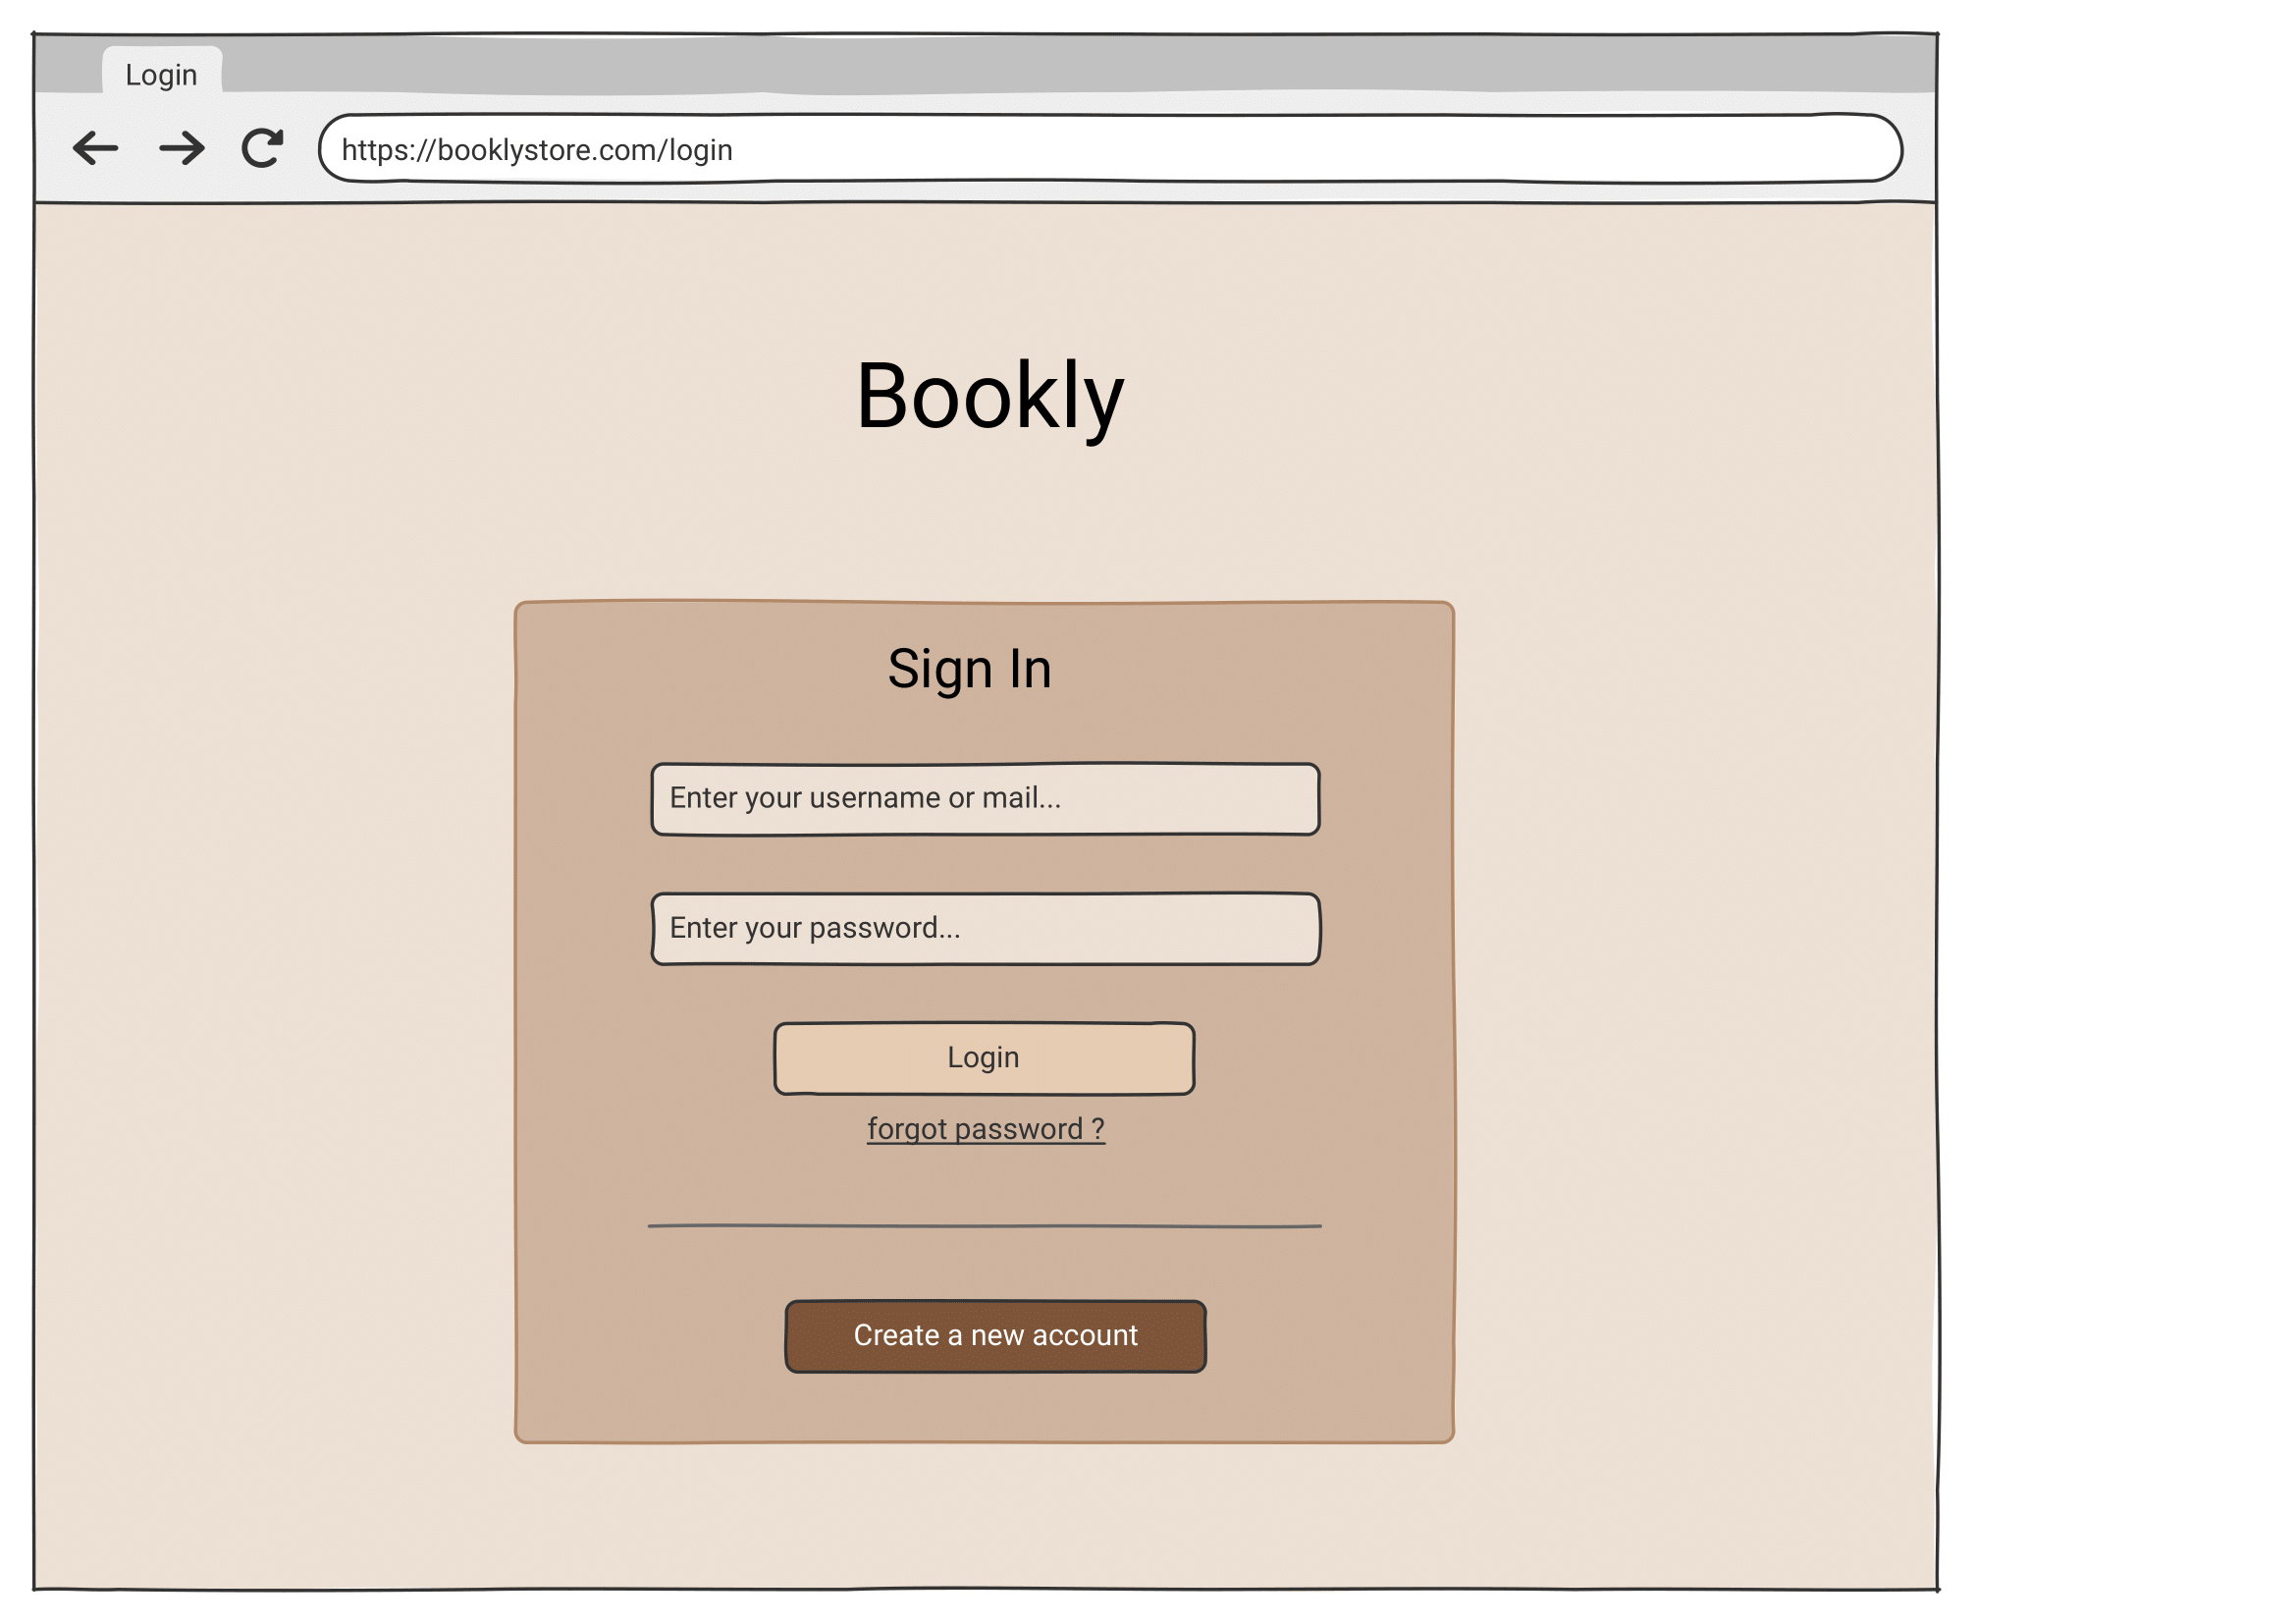
\includegraphics[width=0.6\linewidth]{HW1Report/photos/signin.png}

\begin{figure}[h!]
    \centering
    \caption{sign in page}
    \label{fig:enter-label}
\end{figure}

\label{sec:signin}
This page allows users to either sign in to an existing account or register for a new one.

The \textbf{Sign In section} includes:
\begin{itemize}
    \item Input fields for \textbf{username} and \textbf{password}.
    \item A link for \textbf{password recovery} in case the user forgets their credentials.
    \item A button redirecting new users to the \textbf{Sign Up section}.
\end{itemize}

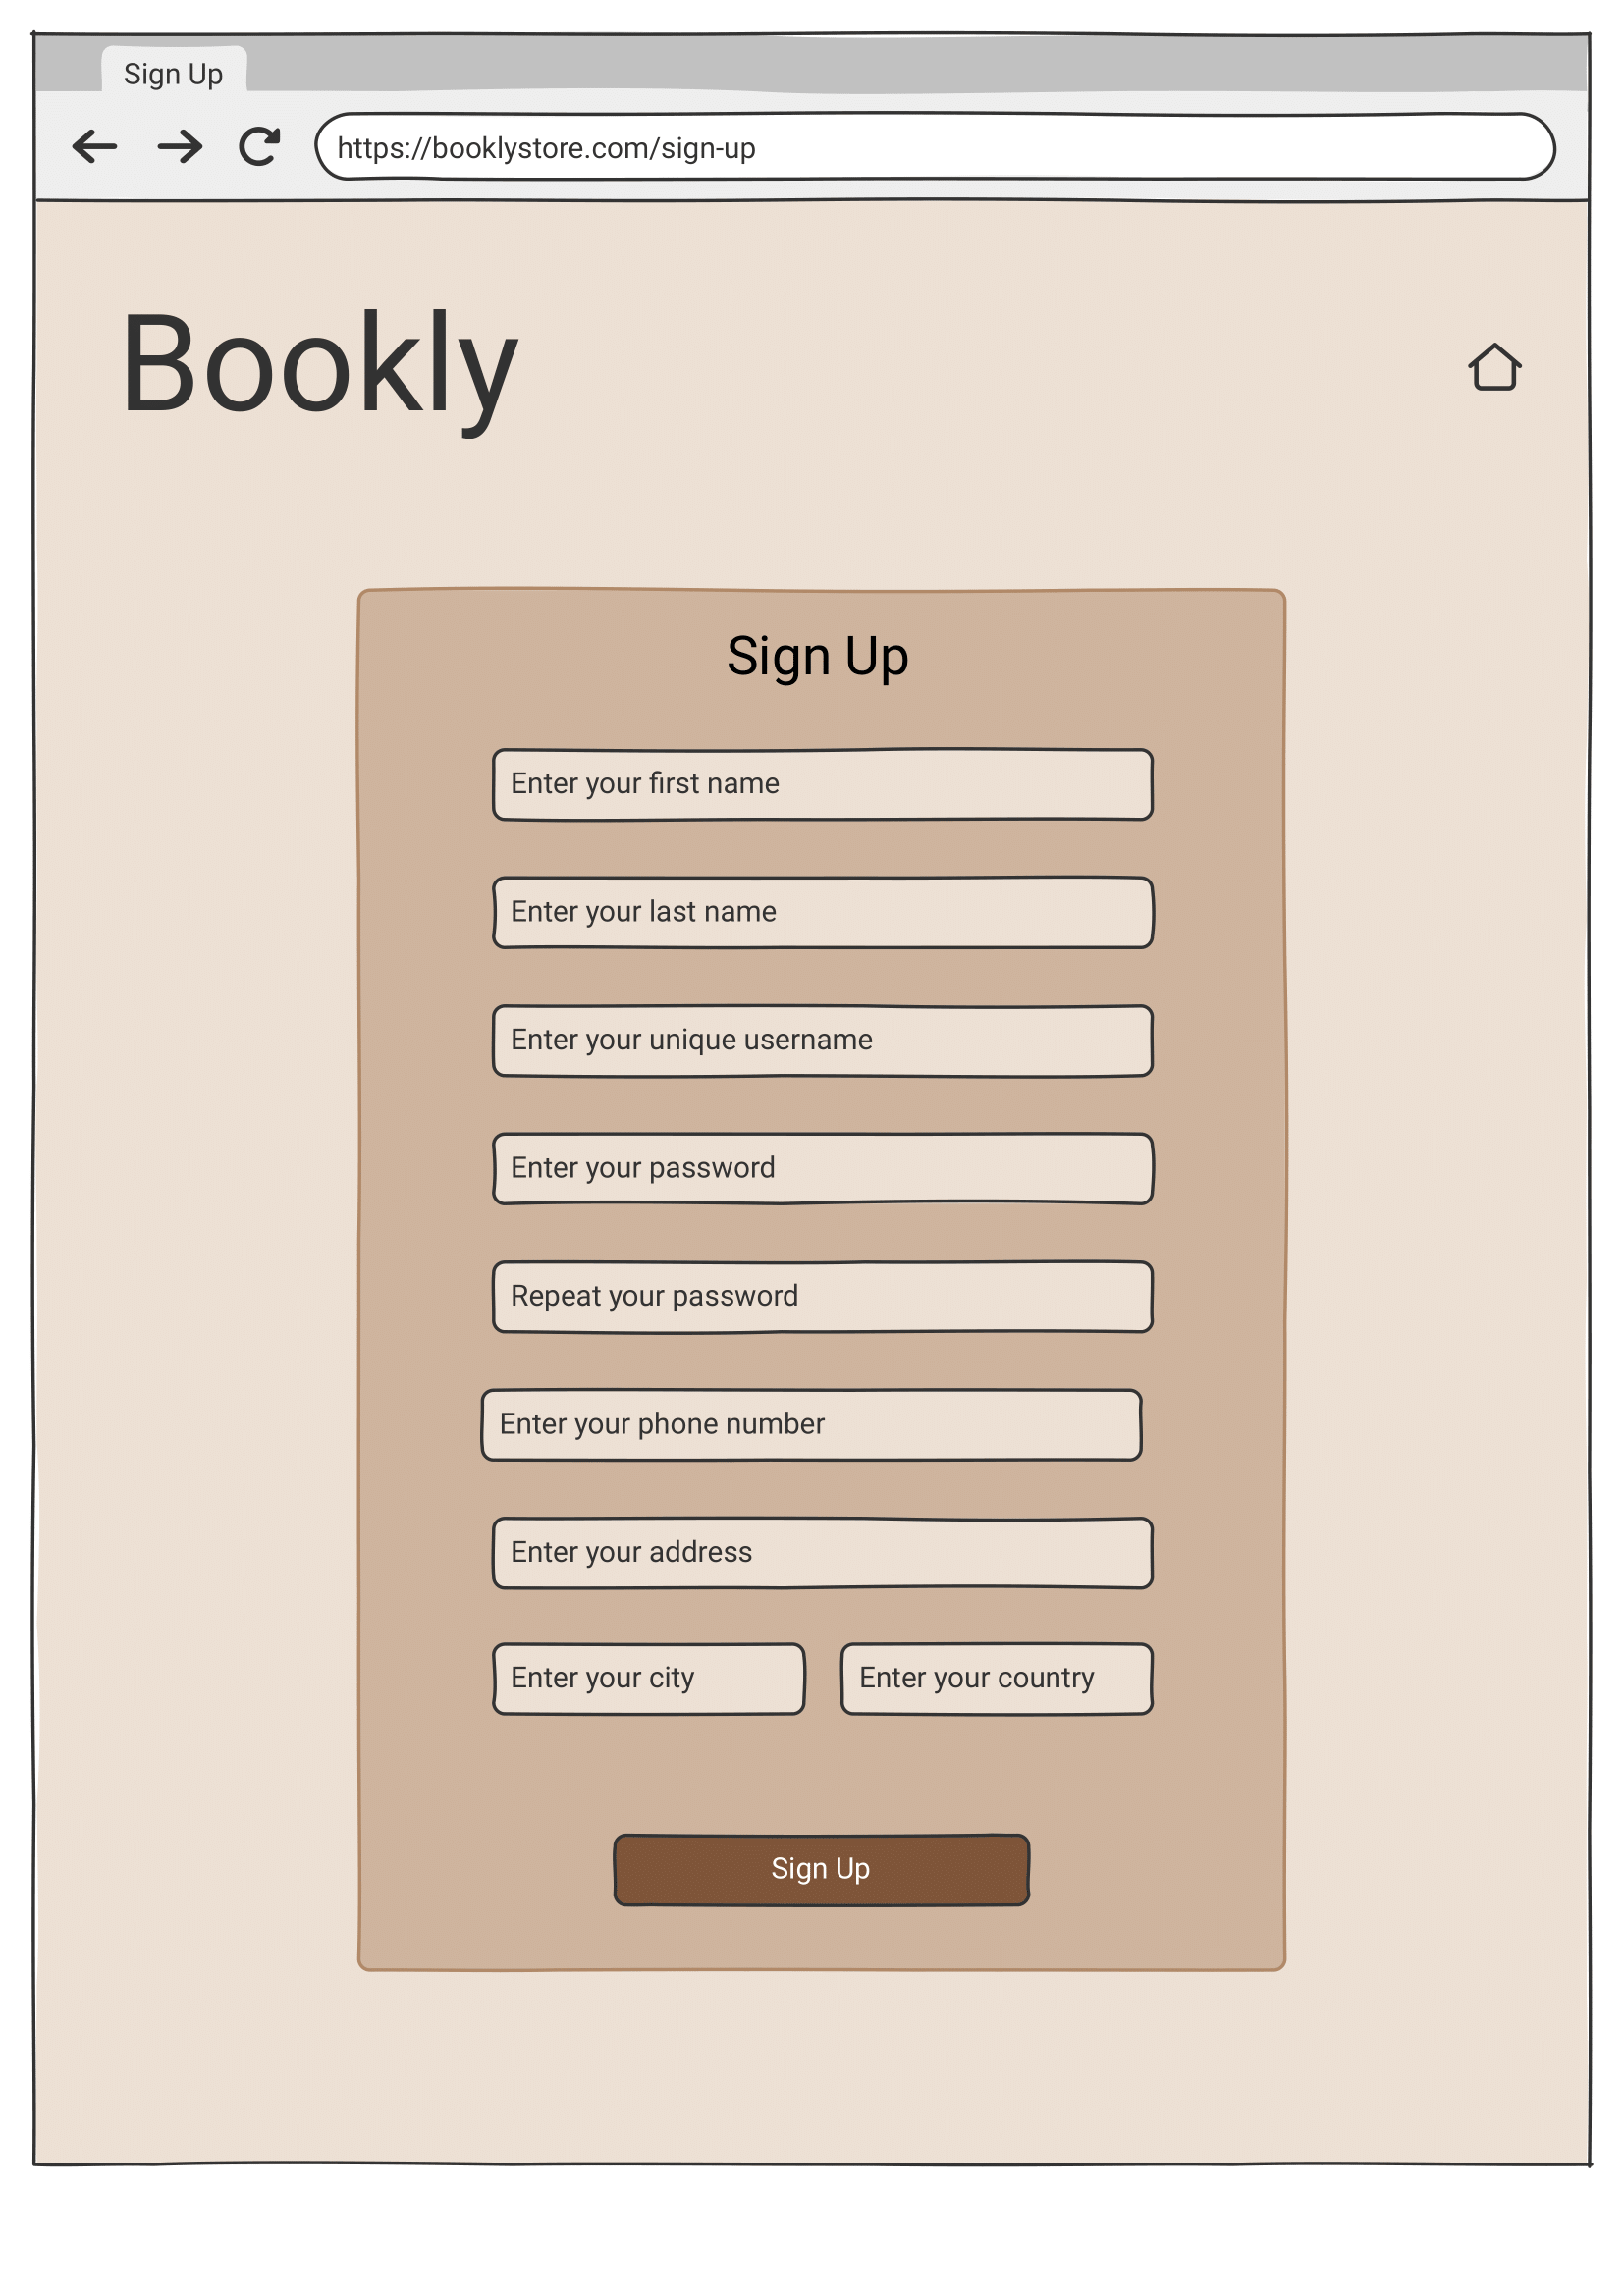
\includegraphics[width=0.6\linewidth]{HW1Report/photos/signup.png}

\begin{figure}[h!]
    \centering
    \caption{sign up page}
    \label{fig:enter-label}
\end{figure}
The \textbf{Sign Up section} provides a registration form with the following input fields:
\begin{itemize}
    \item \textbf{First Name} and \textbf{Last Name}
    \item A unique \textbf{Username}
    \item \textbf{Password}
    \item \textbf{Phone Number}
    \item \textbf{Address}
\end{itemize}


\subsection{User Profile Page} 

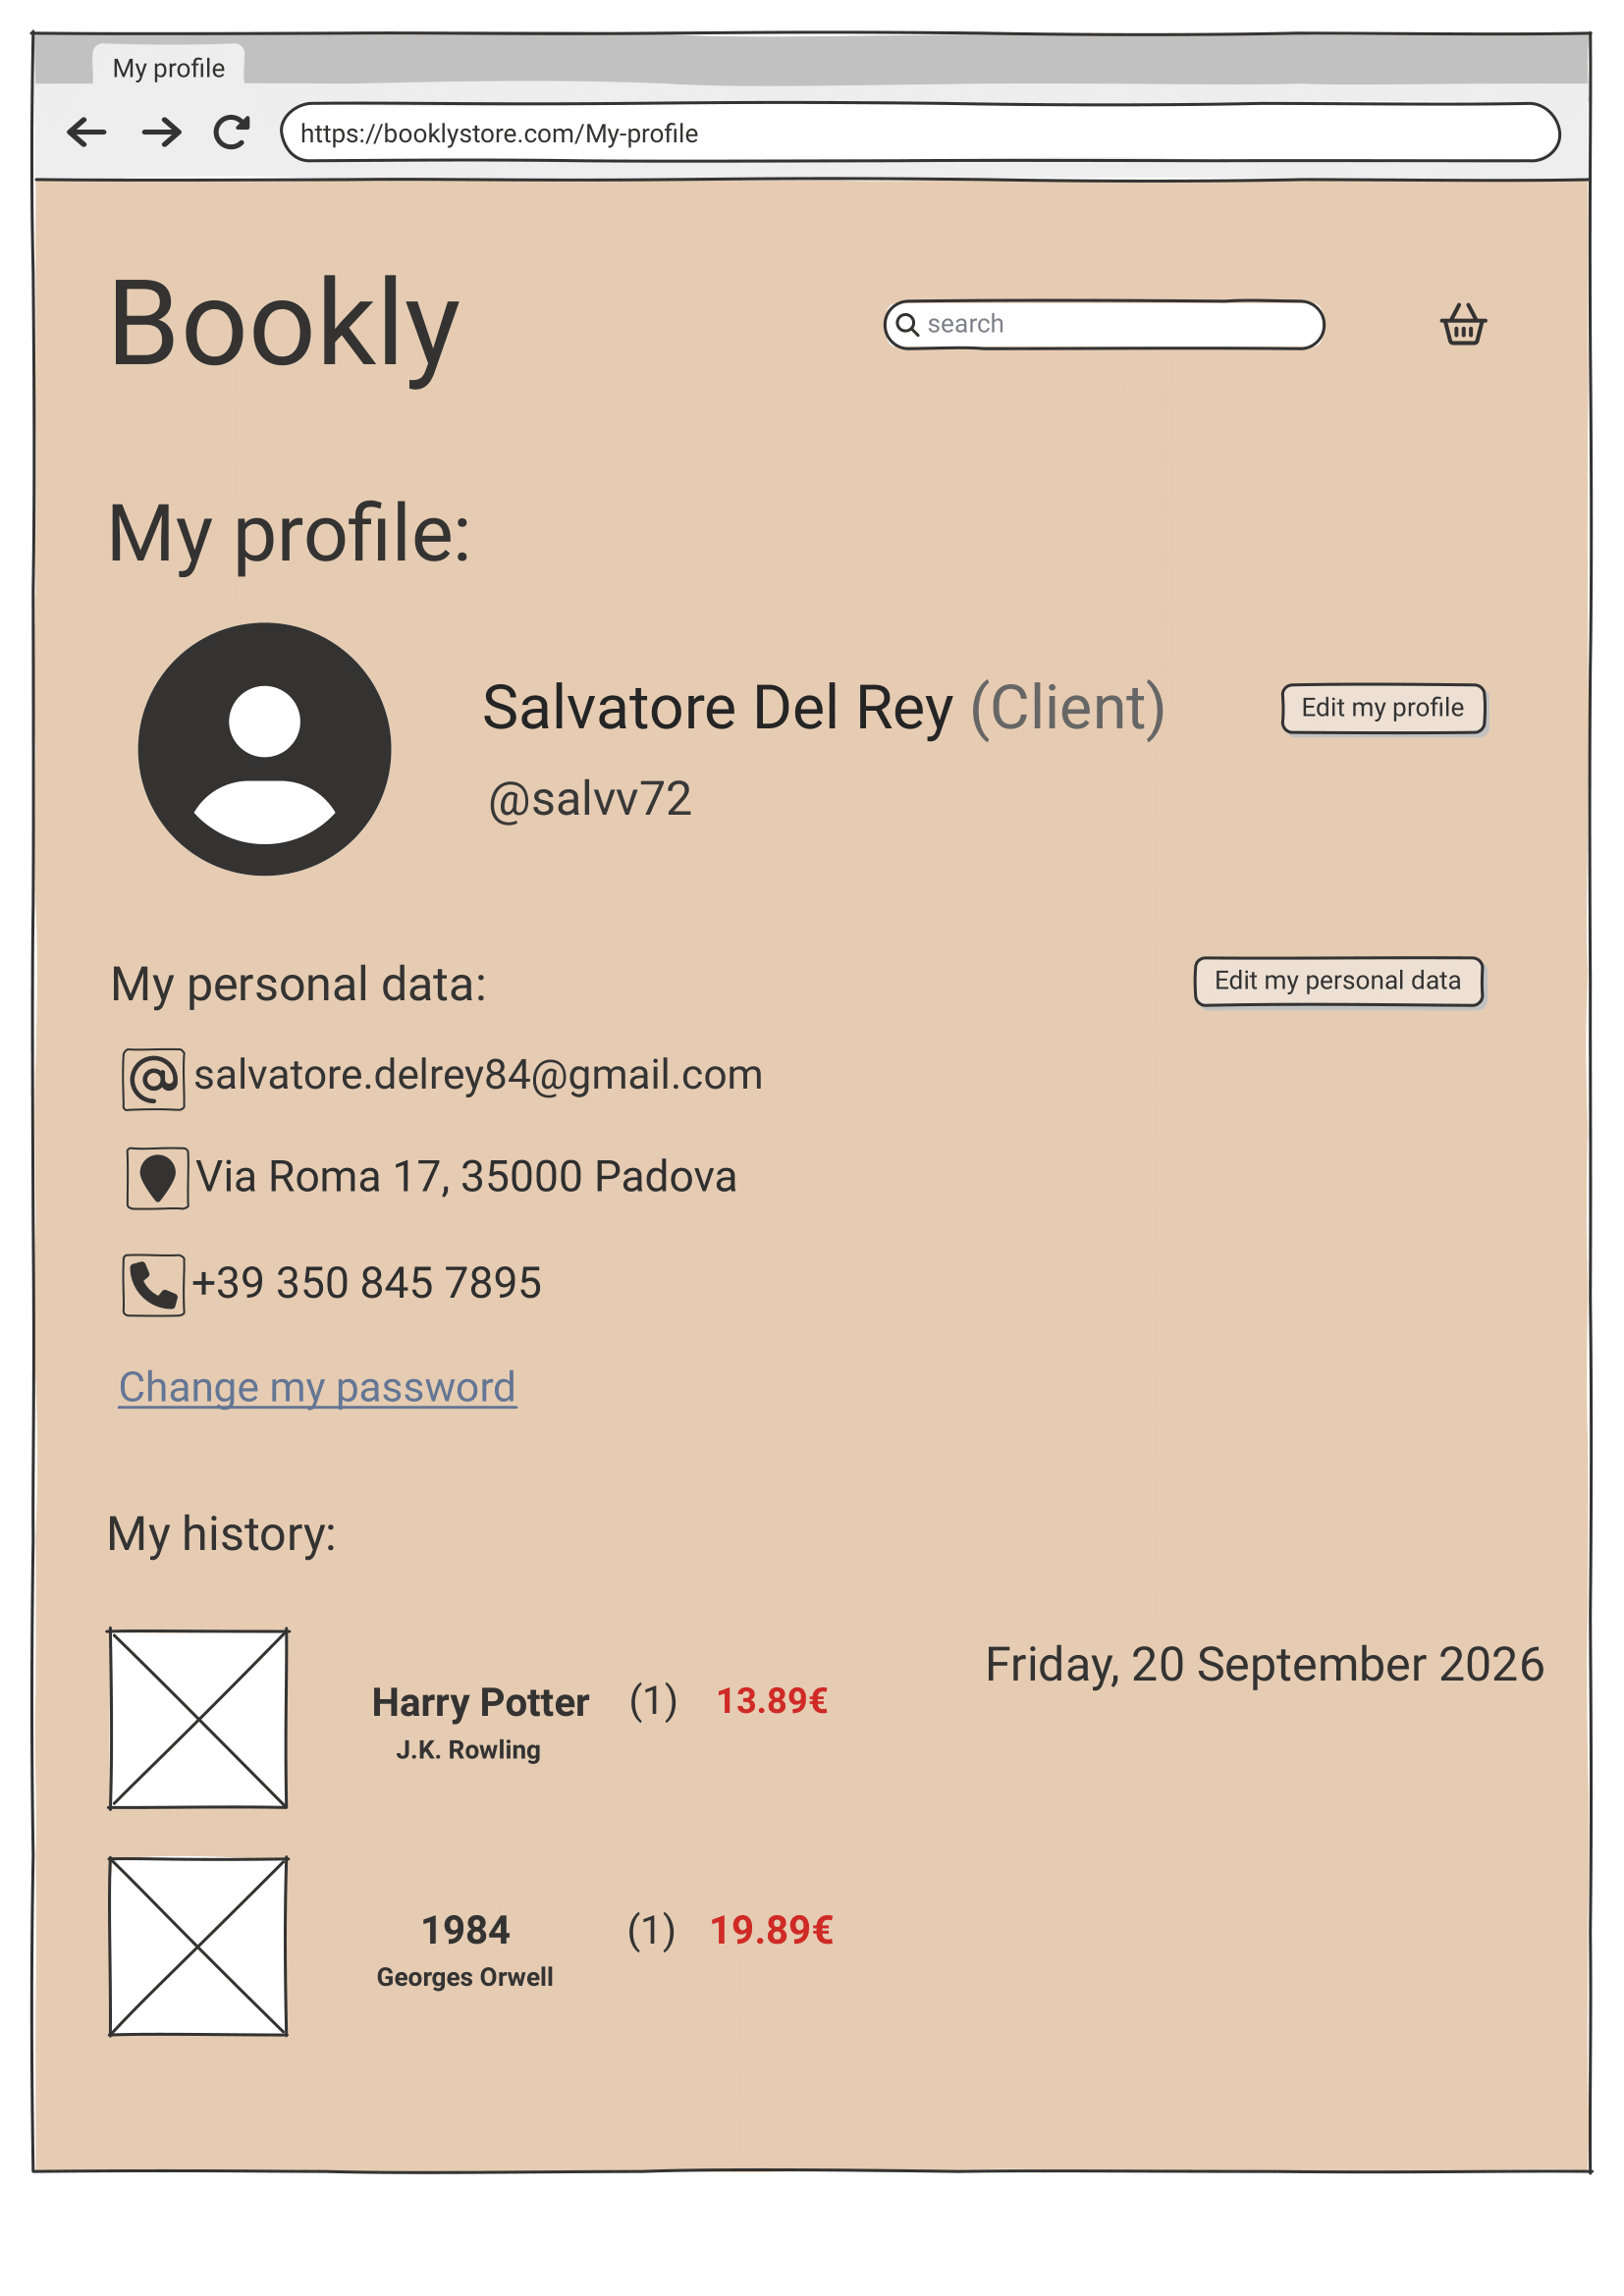
\includegraphics[width=0.6\linewidth]{HW1Report/photos/profilepage2.png}

\begin{figure}[h!]
    \centering
    \caption{profile page}
    \label{fig:enter-label}
\end{figure}

\label{sec:profile}
Users can also access their profile page, which displays their personal details and order history. The page will include the following information:

\begin{itemize}
    \item \textbf{First Name and Last Name}: The full name of the user.
    \item \textbf{Role}: Indicates whether the user is a \textit{Client} or an \textit{Admin}.
    \item \textbf{Username}: A unique identifier for the user within the platform.
    \item \textbf{Email Address}: The registered email associated with the account.
    \item \textbf{Address}: The user's delivery address.
    \item \textbf{Phone Number}: The user's contact number.
\end{itemize}

The page will also provide:
\begin{itemize}
    \item \textbf{Edit Buttons}: Users will have the option to update their personal information through dedicated buttons.
    \item \textbf{Change Password Link}: A dynamic text link labeled \textit{"Change my password"} that, when clicked, redirects users to a dedicated password update page.
\end{itemize}


\subsection{Book Page} \label{sec:book}

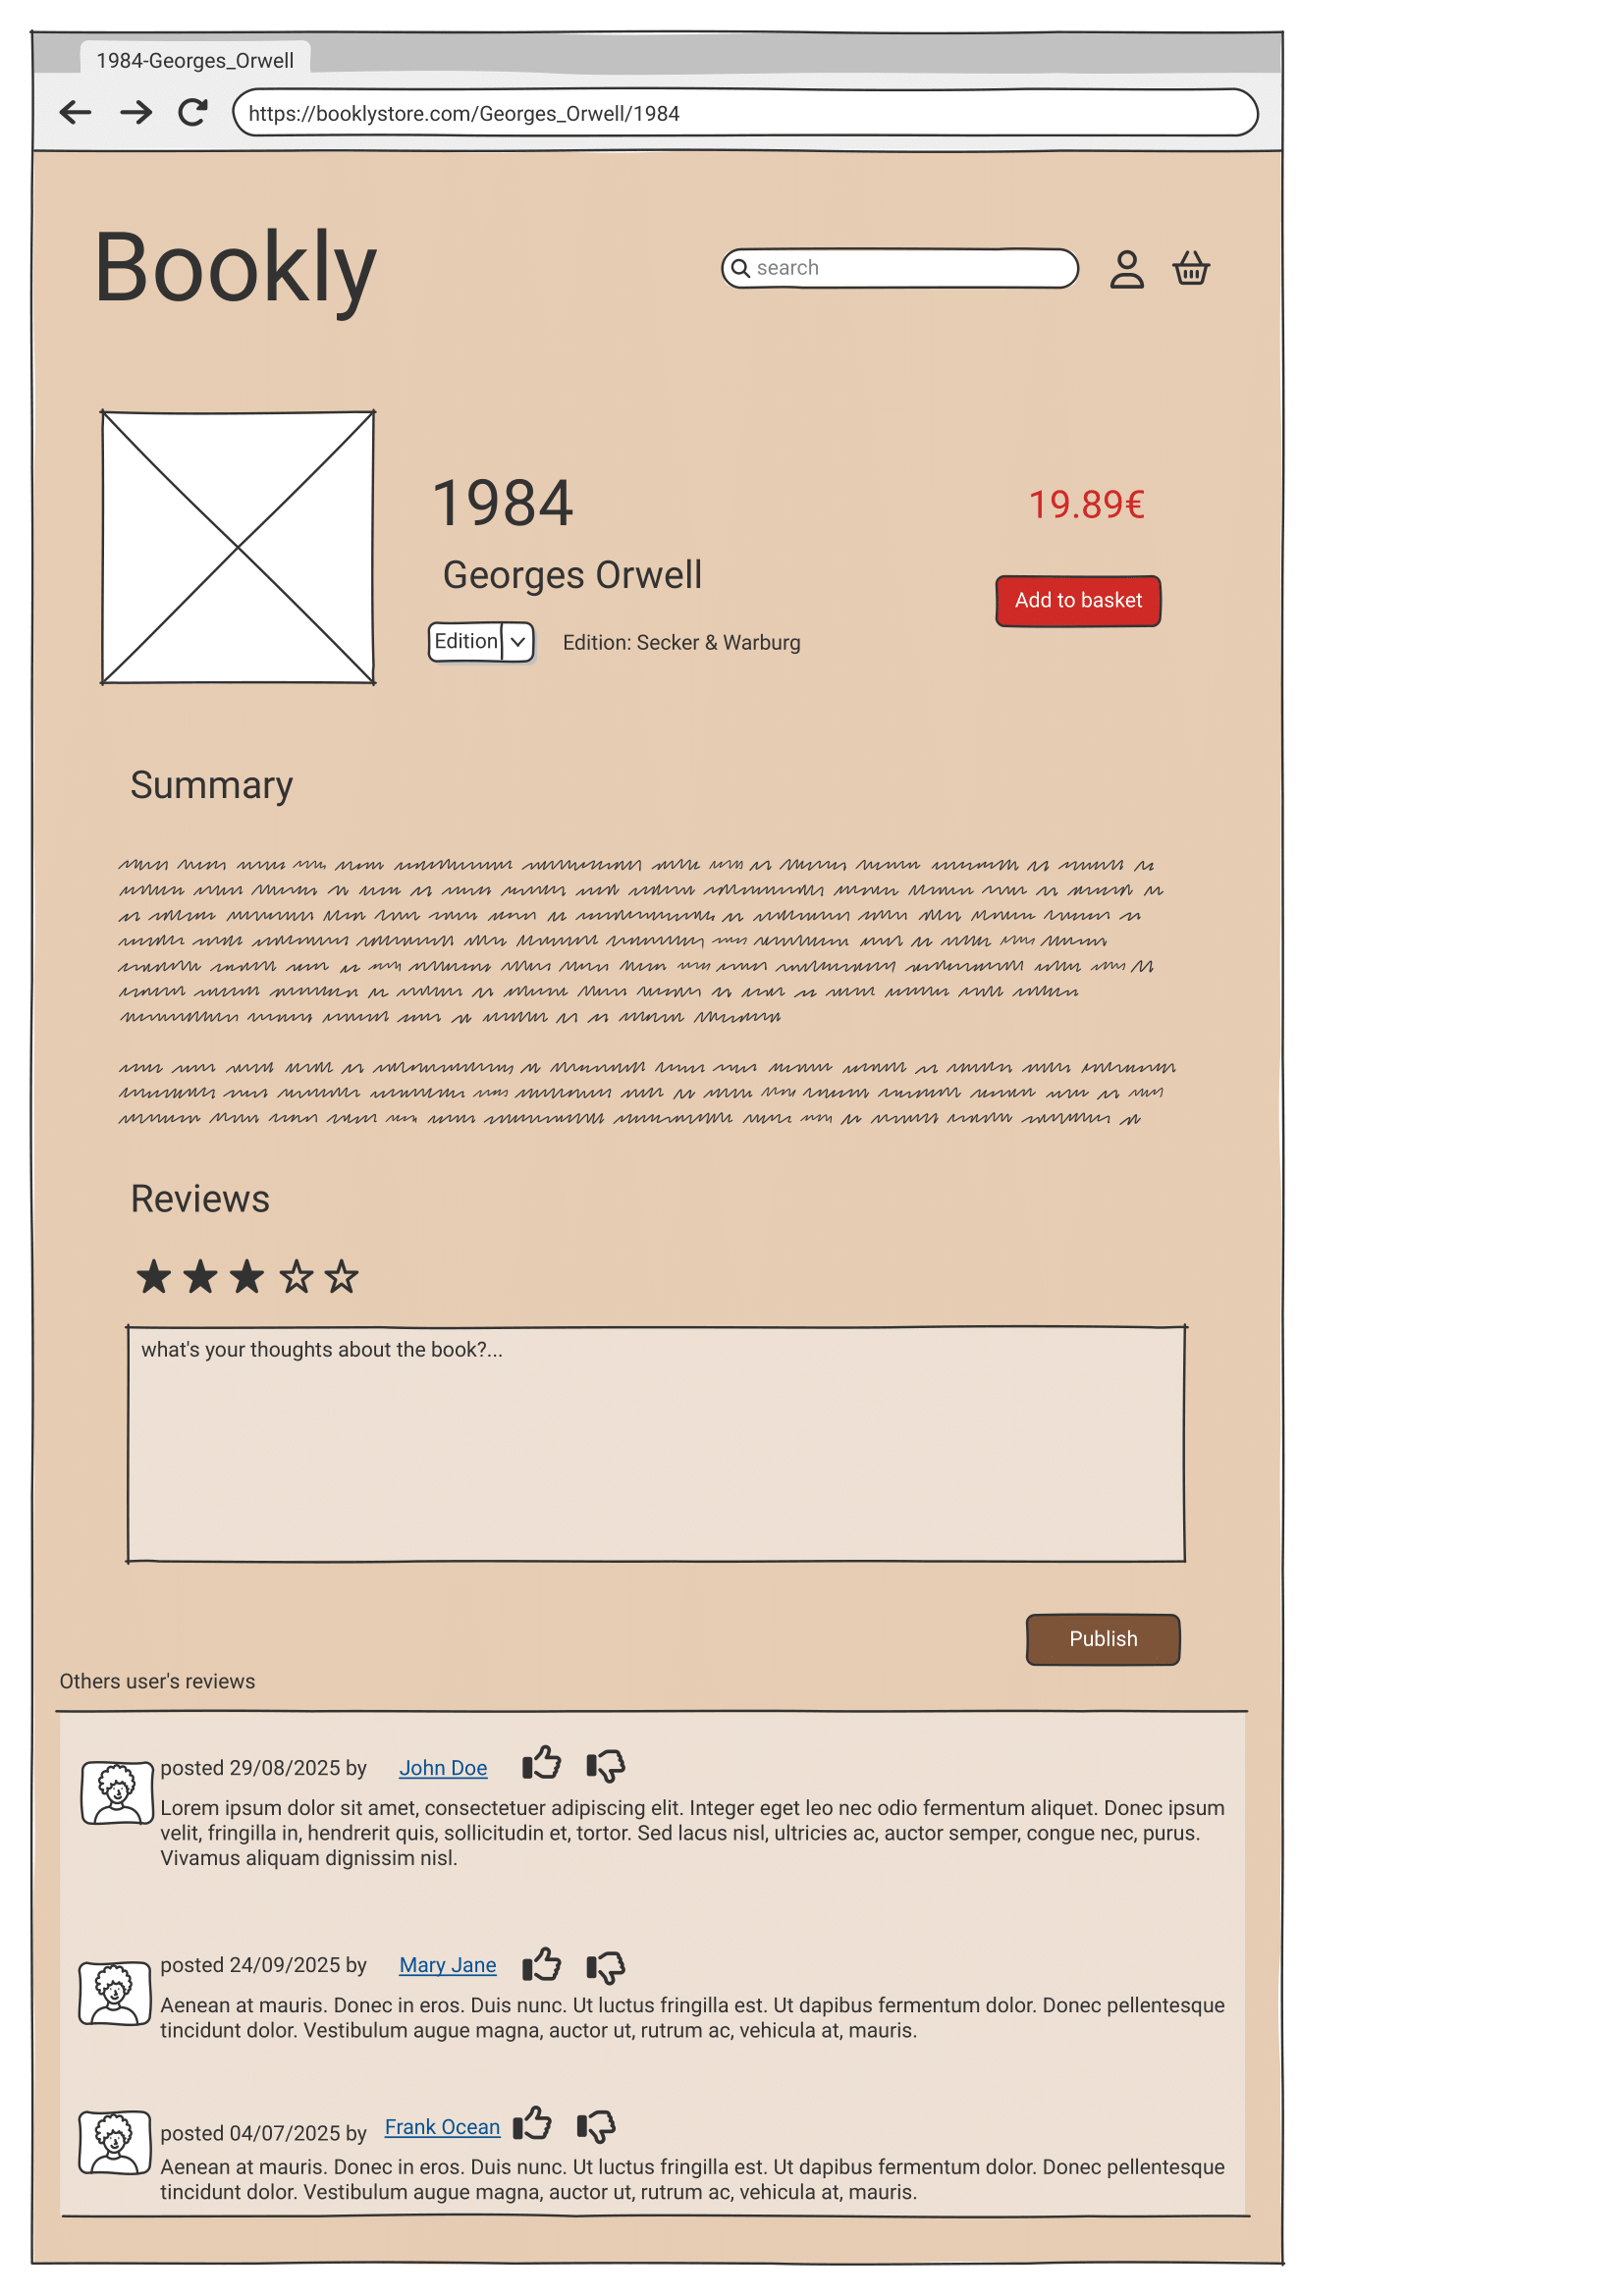
\includegraphics[width=0.6\linewidth]{HW1Report/photos/bookpage2.png}

\begin{figure}[h!]
    \centering
    \caption{book page}
    \label{fig:enter-label}
\end{figure}
Each book will have its own dedicated page containing the following details: \textbf{Title}, \textbf{Author}, \textbf{Price}, \textbf{Edition}, \textbf{Genre}, \textbf{Summary} and a \textbf{cover image} of the book.

In top of that, the page will also have:
\begin{itemize}
    \item A \textbf{Review Section}, where users can:
    \begin{itemize}
        \item Like or dislike existing reviews.
        \item Add their own review by writing a comment and rating the book on a scale from \textbf{0 to 5 stars}.
    \end{itemize}
    \item A \textbf{"Add to basket"} button, allowing users to purchase the book.
    \item A \textbf{"Add to wishlist"} button, allowing users to save the book on their wishlist.
\end{itemize}



\subsection{Basket Page} \label{sec:basket}

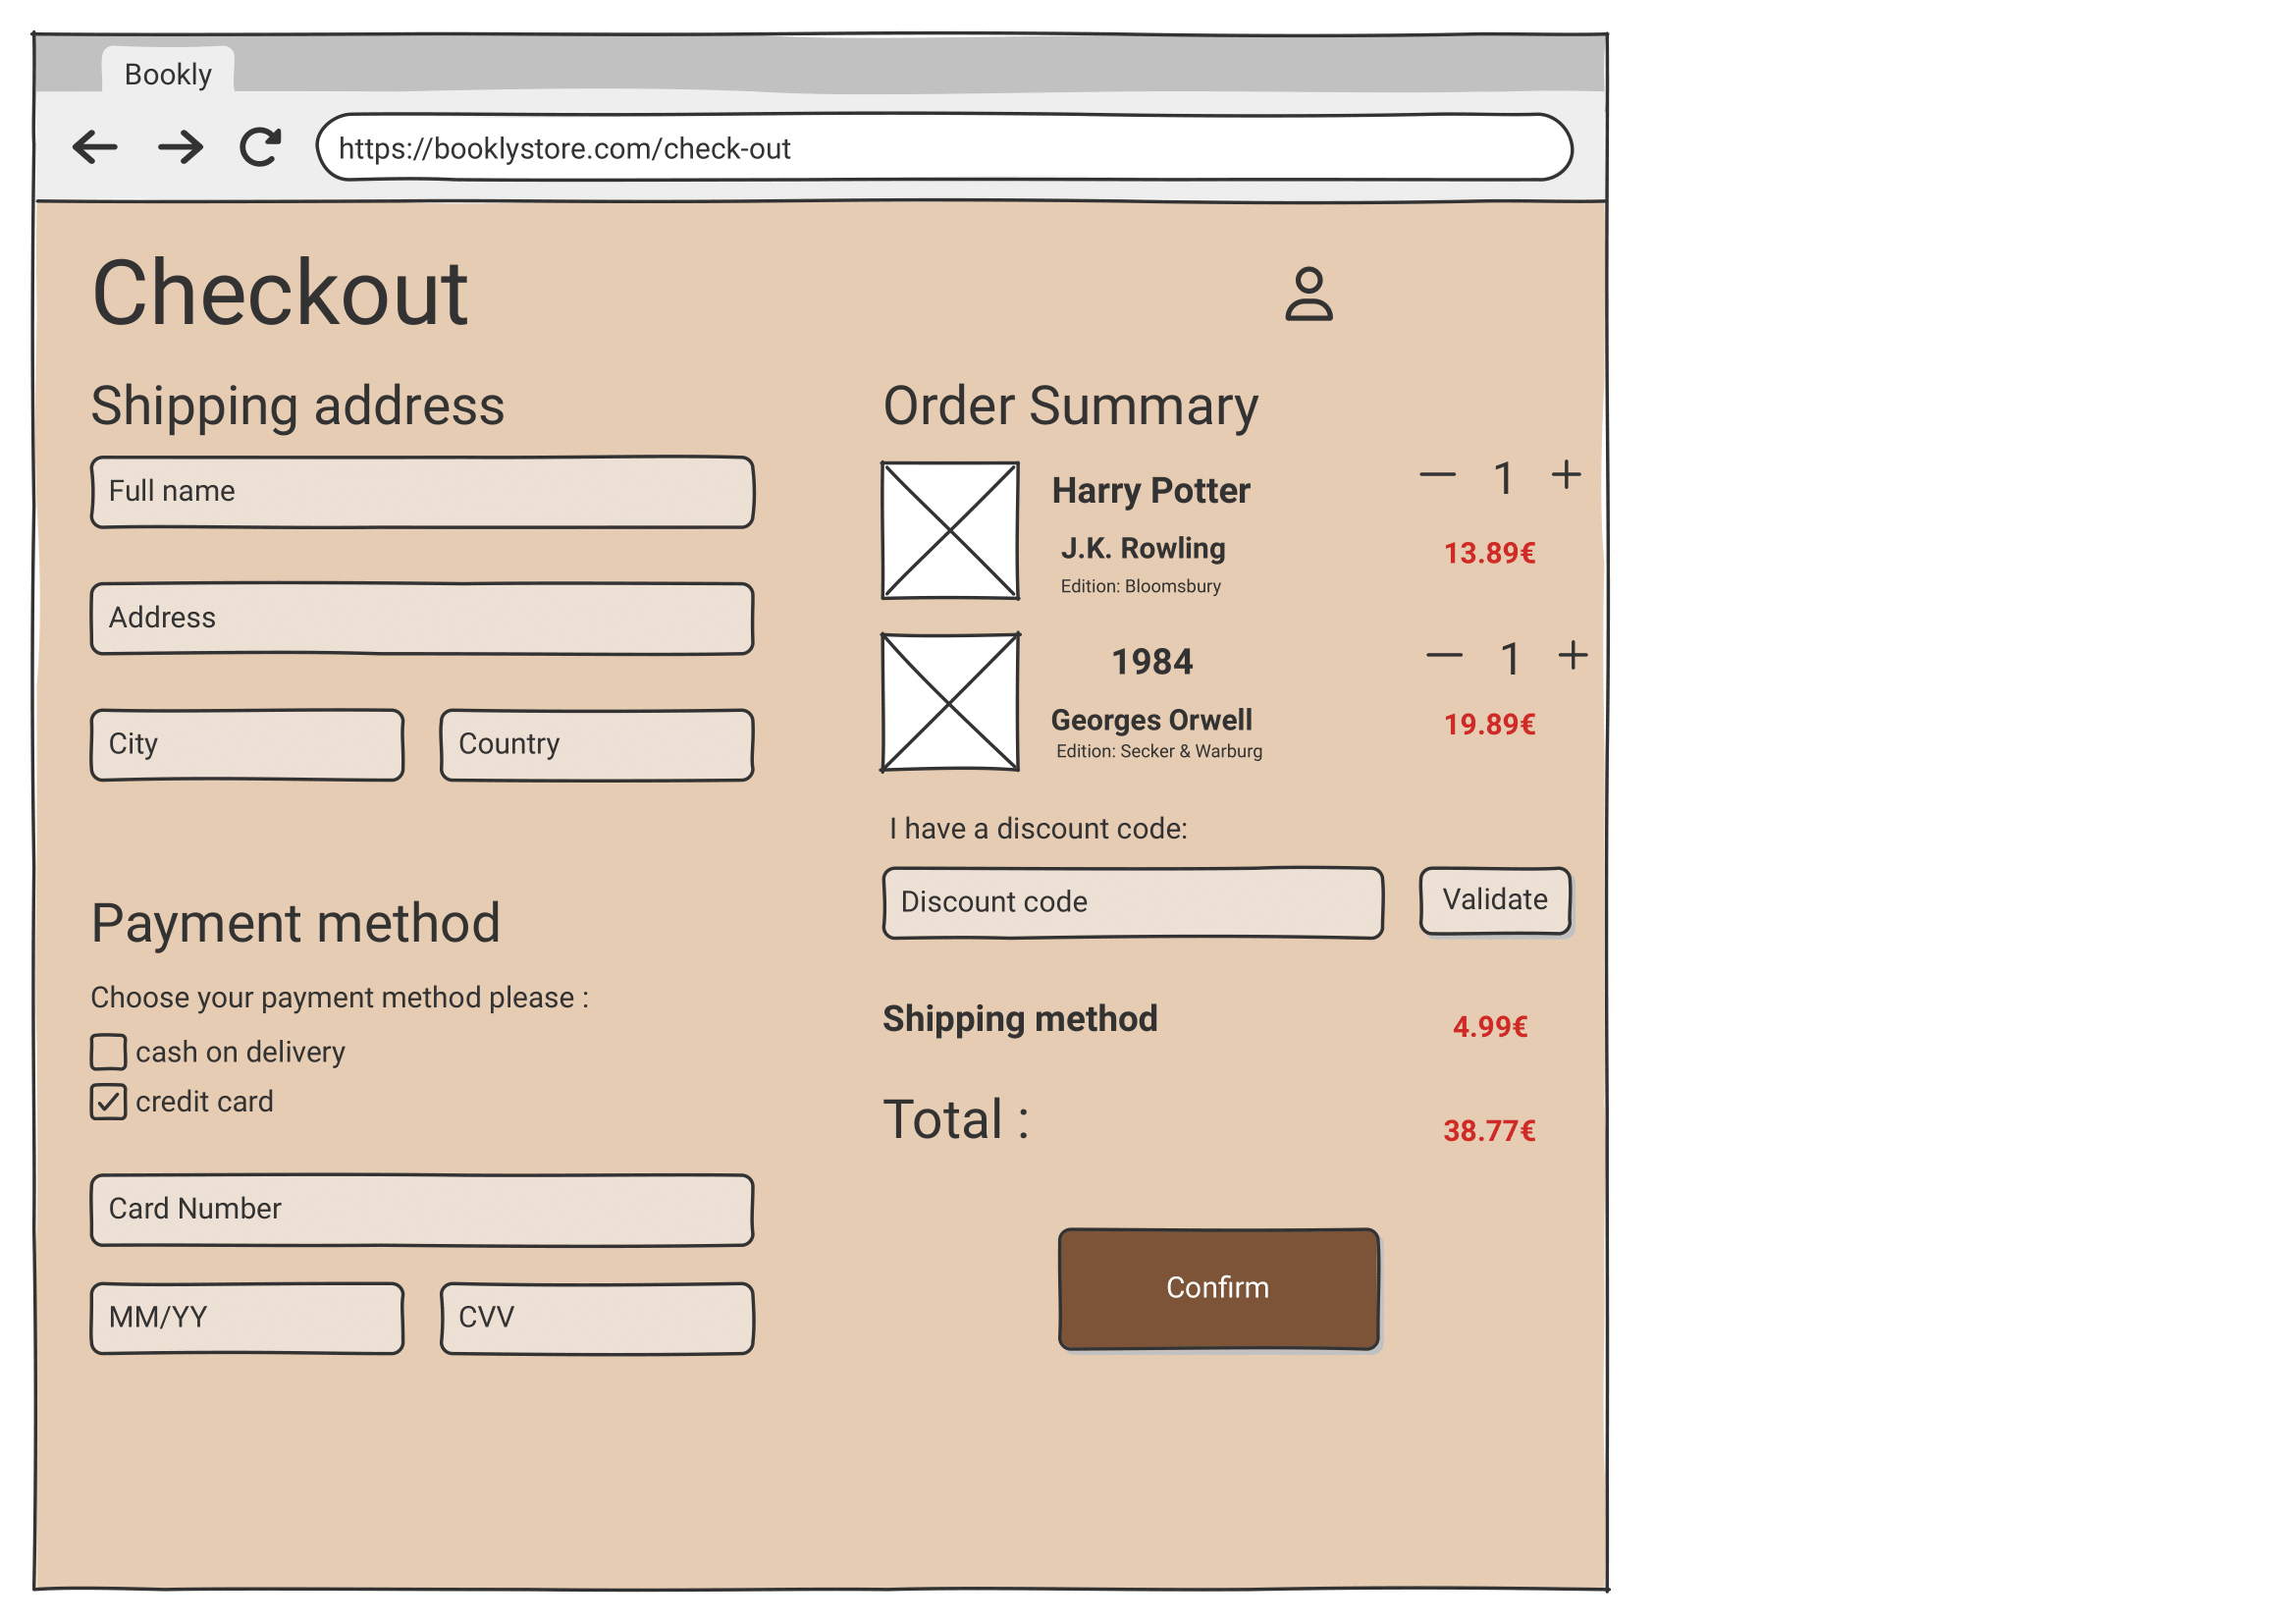
\includegraphics[width=0.6\linewidth]{HW1Report/photos/checkout2.png}

\begin{figure}[h!]
    \centering
    \caption{basket page}
    \label{fig:enter-label}
\end{figure}

This page will display the books added on the basket by the user, along with options to update quantities. It will also include the following features:

\begin{itemize}
    \item A \textbf{recap of all selected books}, displaying their titles, prices, and quantities.
    \item The \textbf{total price}, dynamically updated based on the selected books, their quantities, and the shipping price.
    \item Several input fields for the user to enter their \textbf{billing address}.
    \item A \textbf{payment method selection}, offering the choice between:
    \begin{itemize}
        \item \textbf{Credit/Debit Card Payment}.
        \item \textbf{Cash on Delivery}.
    \end{itemize}
    \item An optional input field for entering a \textbf{discount code} if the user has one.
    \item A \textbf{"Confirm Order"} button that finalizes the payment and processes the order once all required fields are completed.
\end{itemize}


\subsection{Search Results Page} \label{sec:search}

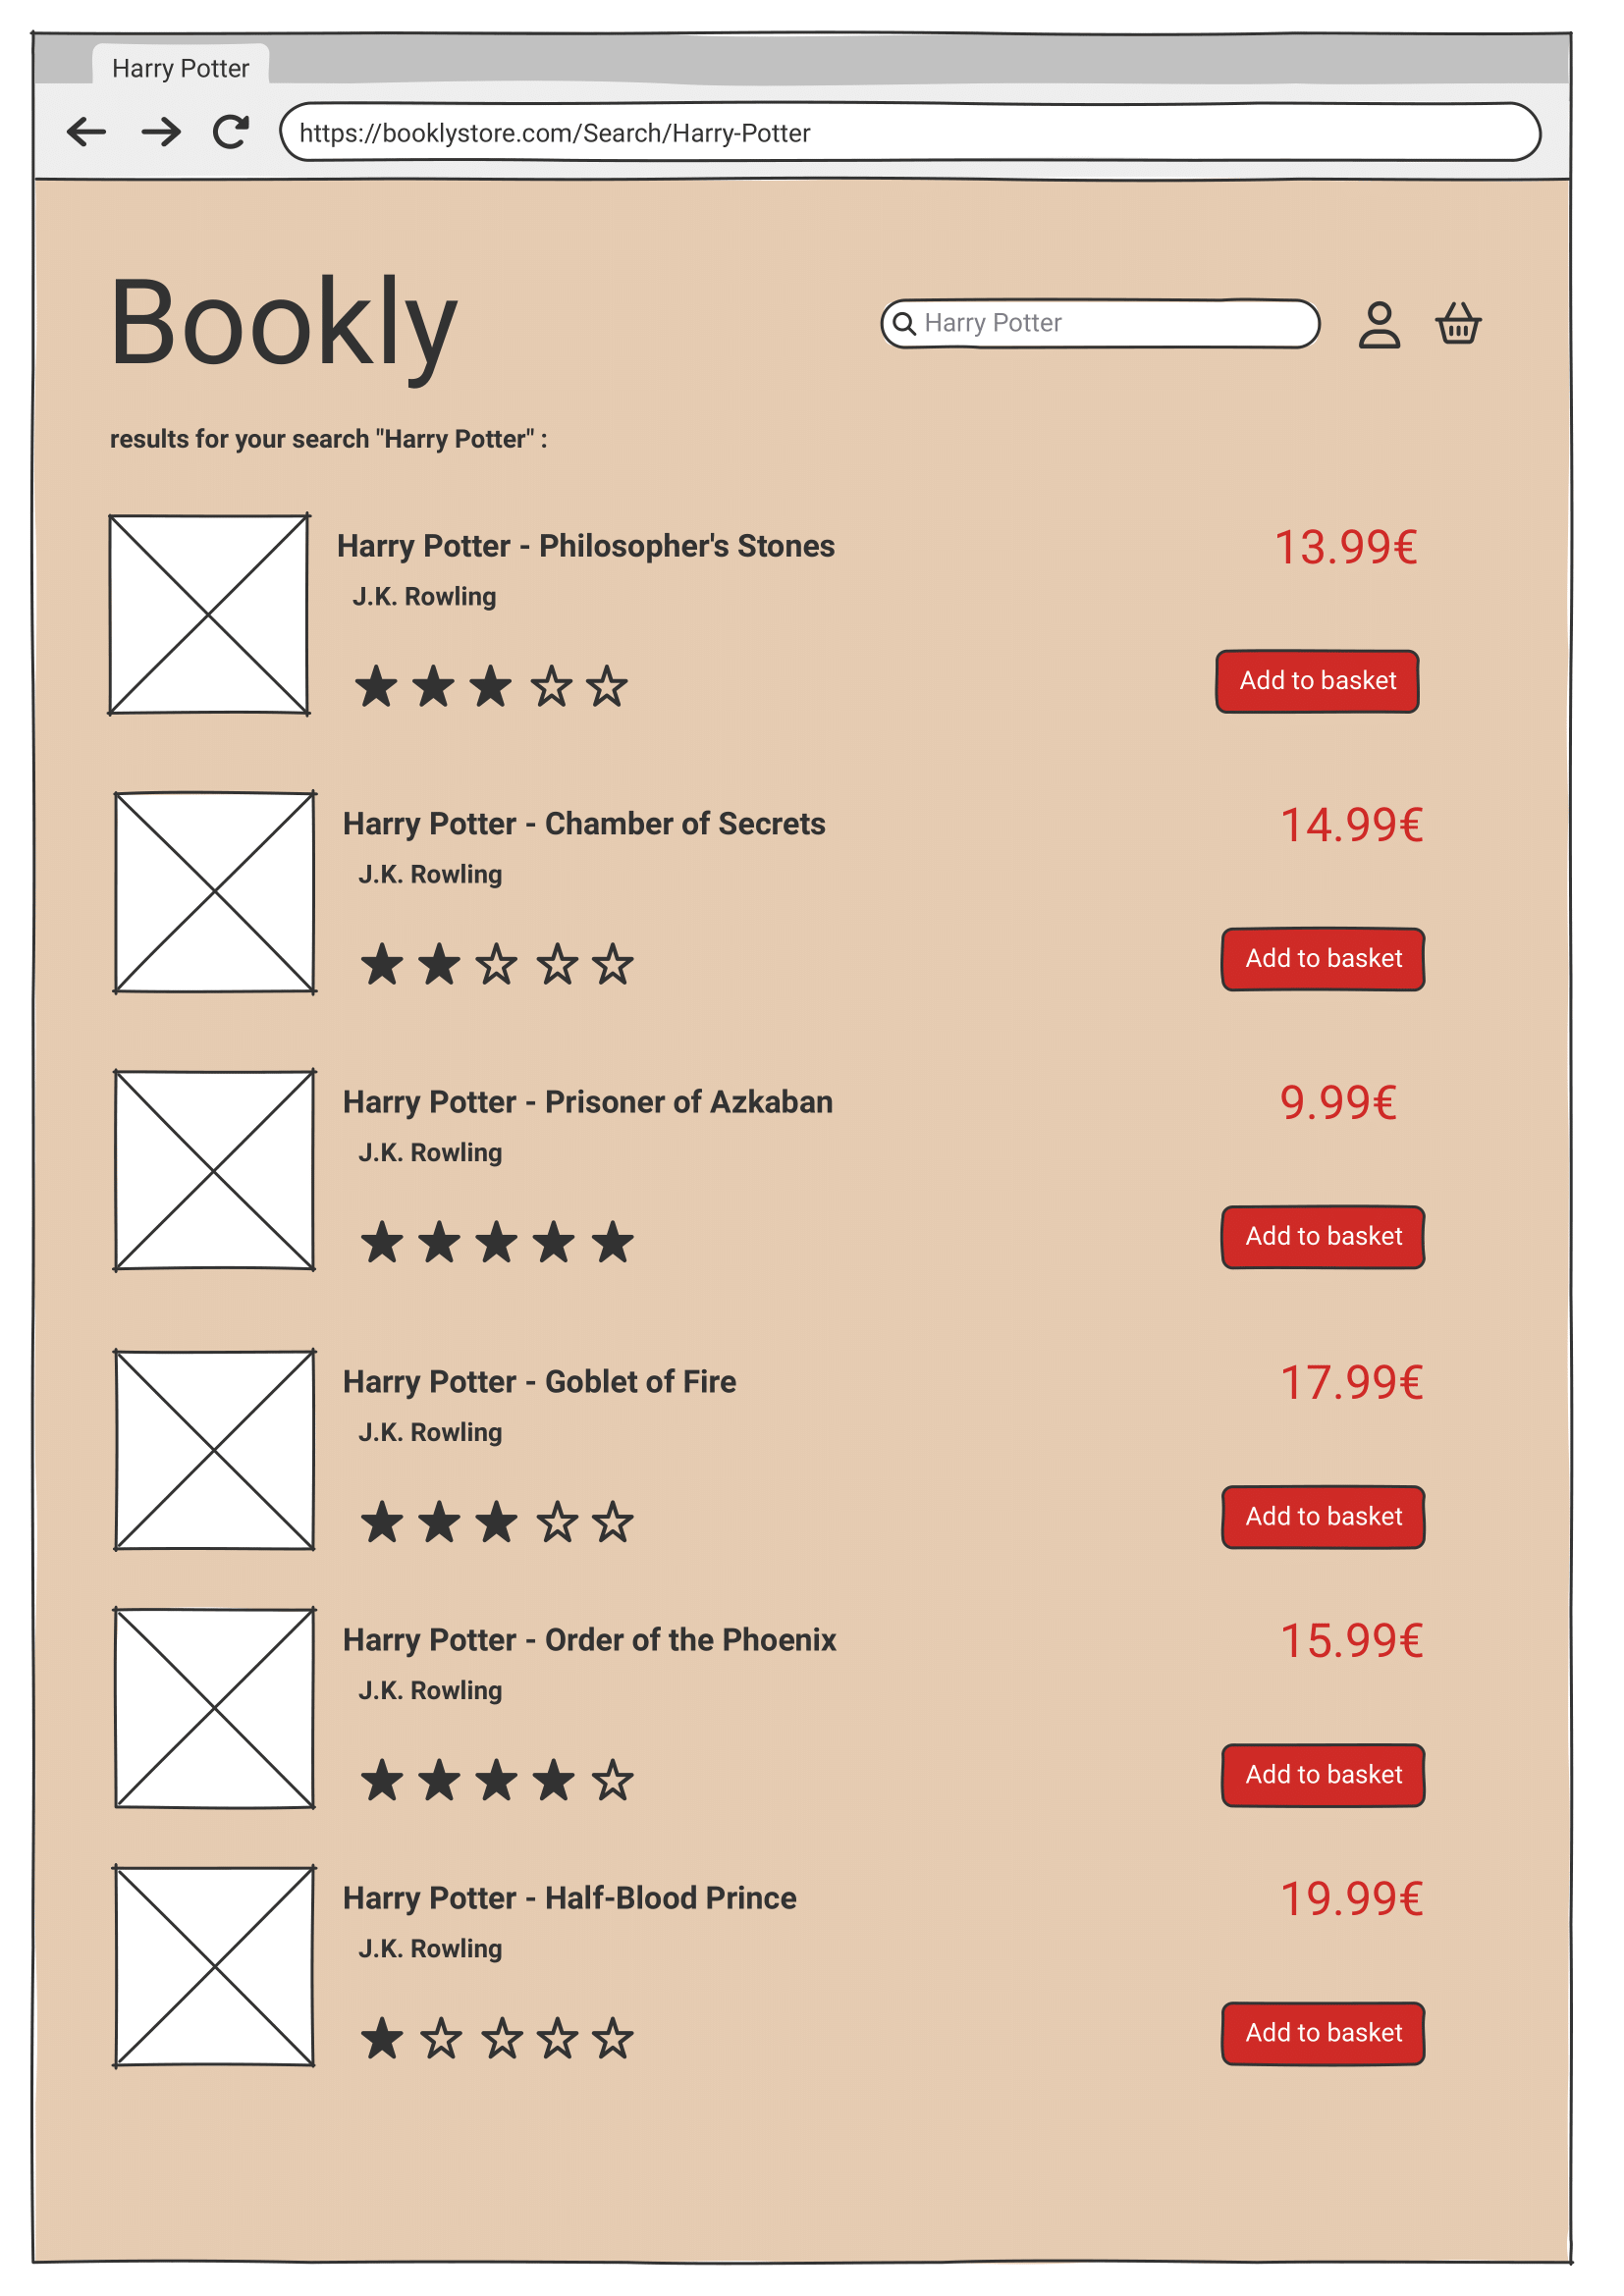
\includegraphics[width=0.6\linewidth]{HW1Report/photos/searchpage.png}

\begin{figure}[h!]
    \centering
    \caption{search page}
    \label{fig:enter-label}
\end{figure}

When a user enters a query in the search bar, they will be redirected to this page, where relevant books will be displayed based on title, author, or genre.

For each book displayed in the search results, the following details will be shown:
\begin{itemize}
    \item The \textbf{book title} and \textbf{cover image}, both acting as clickable links that redirect to the corresponding \hyperref[sec:book]{Book Page}.
    \item The \textbf{average rating}, displayed as a star rating out of 5, based on user reviews.
    \item A \textbf{"Add to Basket"} button along with the corresponding price of the book, allowing users to quickly add the book to their shopping cart.
\end{itemize}

\subsection{Author Page} \label{sec:author}
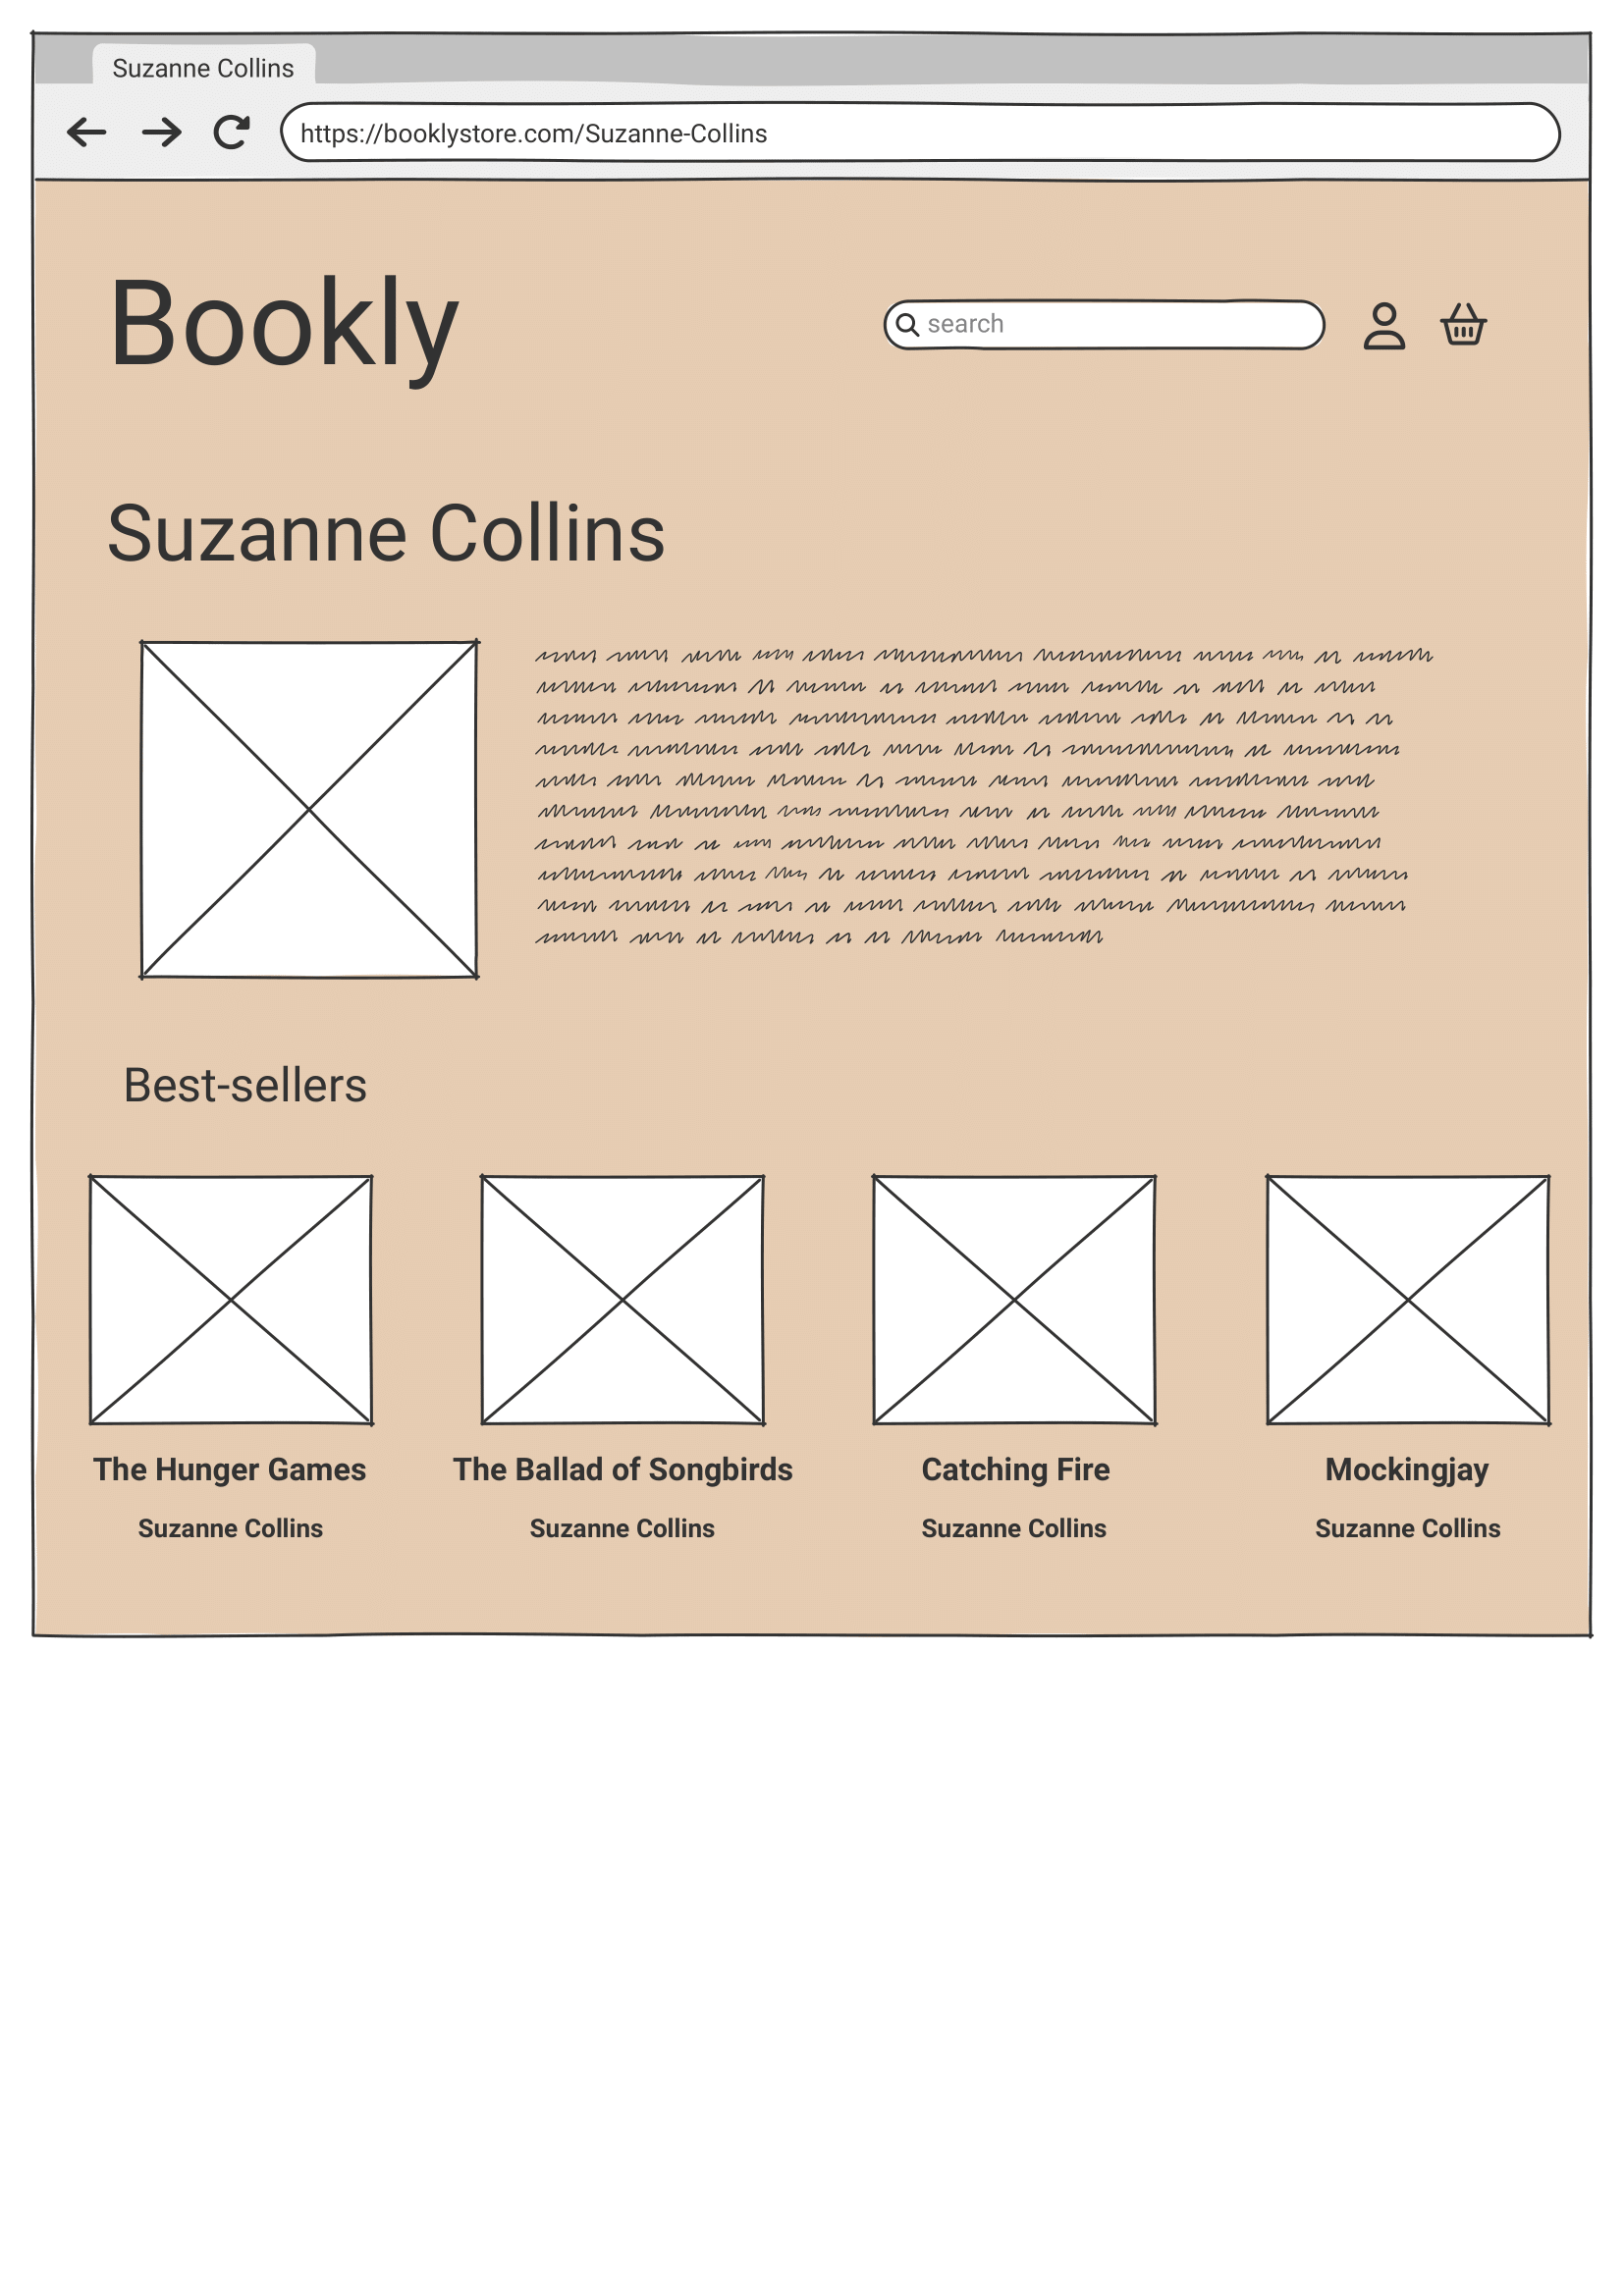
\includegraphics[width=0.6\linewidth]{HW1Report/photos/AuthorPage.png}

\begin{figure}[h!]
    \centering
    \caption{author page}
    \label{fig:enter-label}
\end{figure}

Each author will have his own dedicated page displaying their full name, biography, and literary background. This page will help users explore more books from the same author by displaying their best-sellers.


\subsection{order Page} \label{sec:cart}
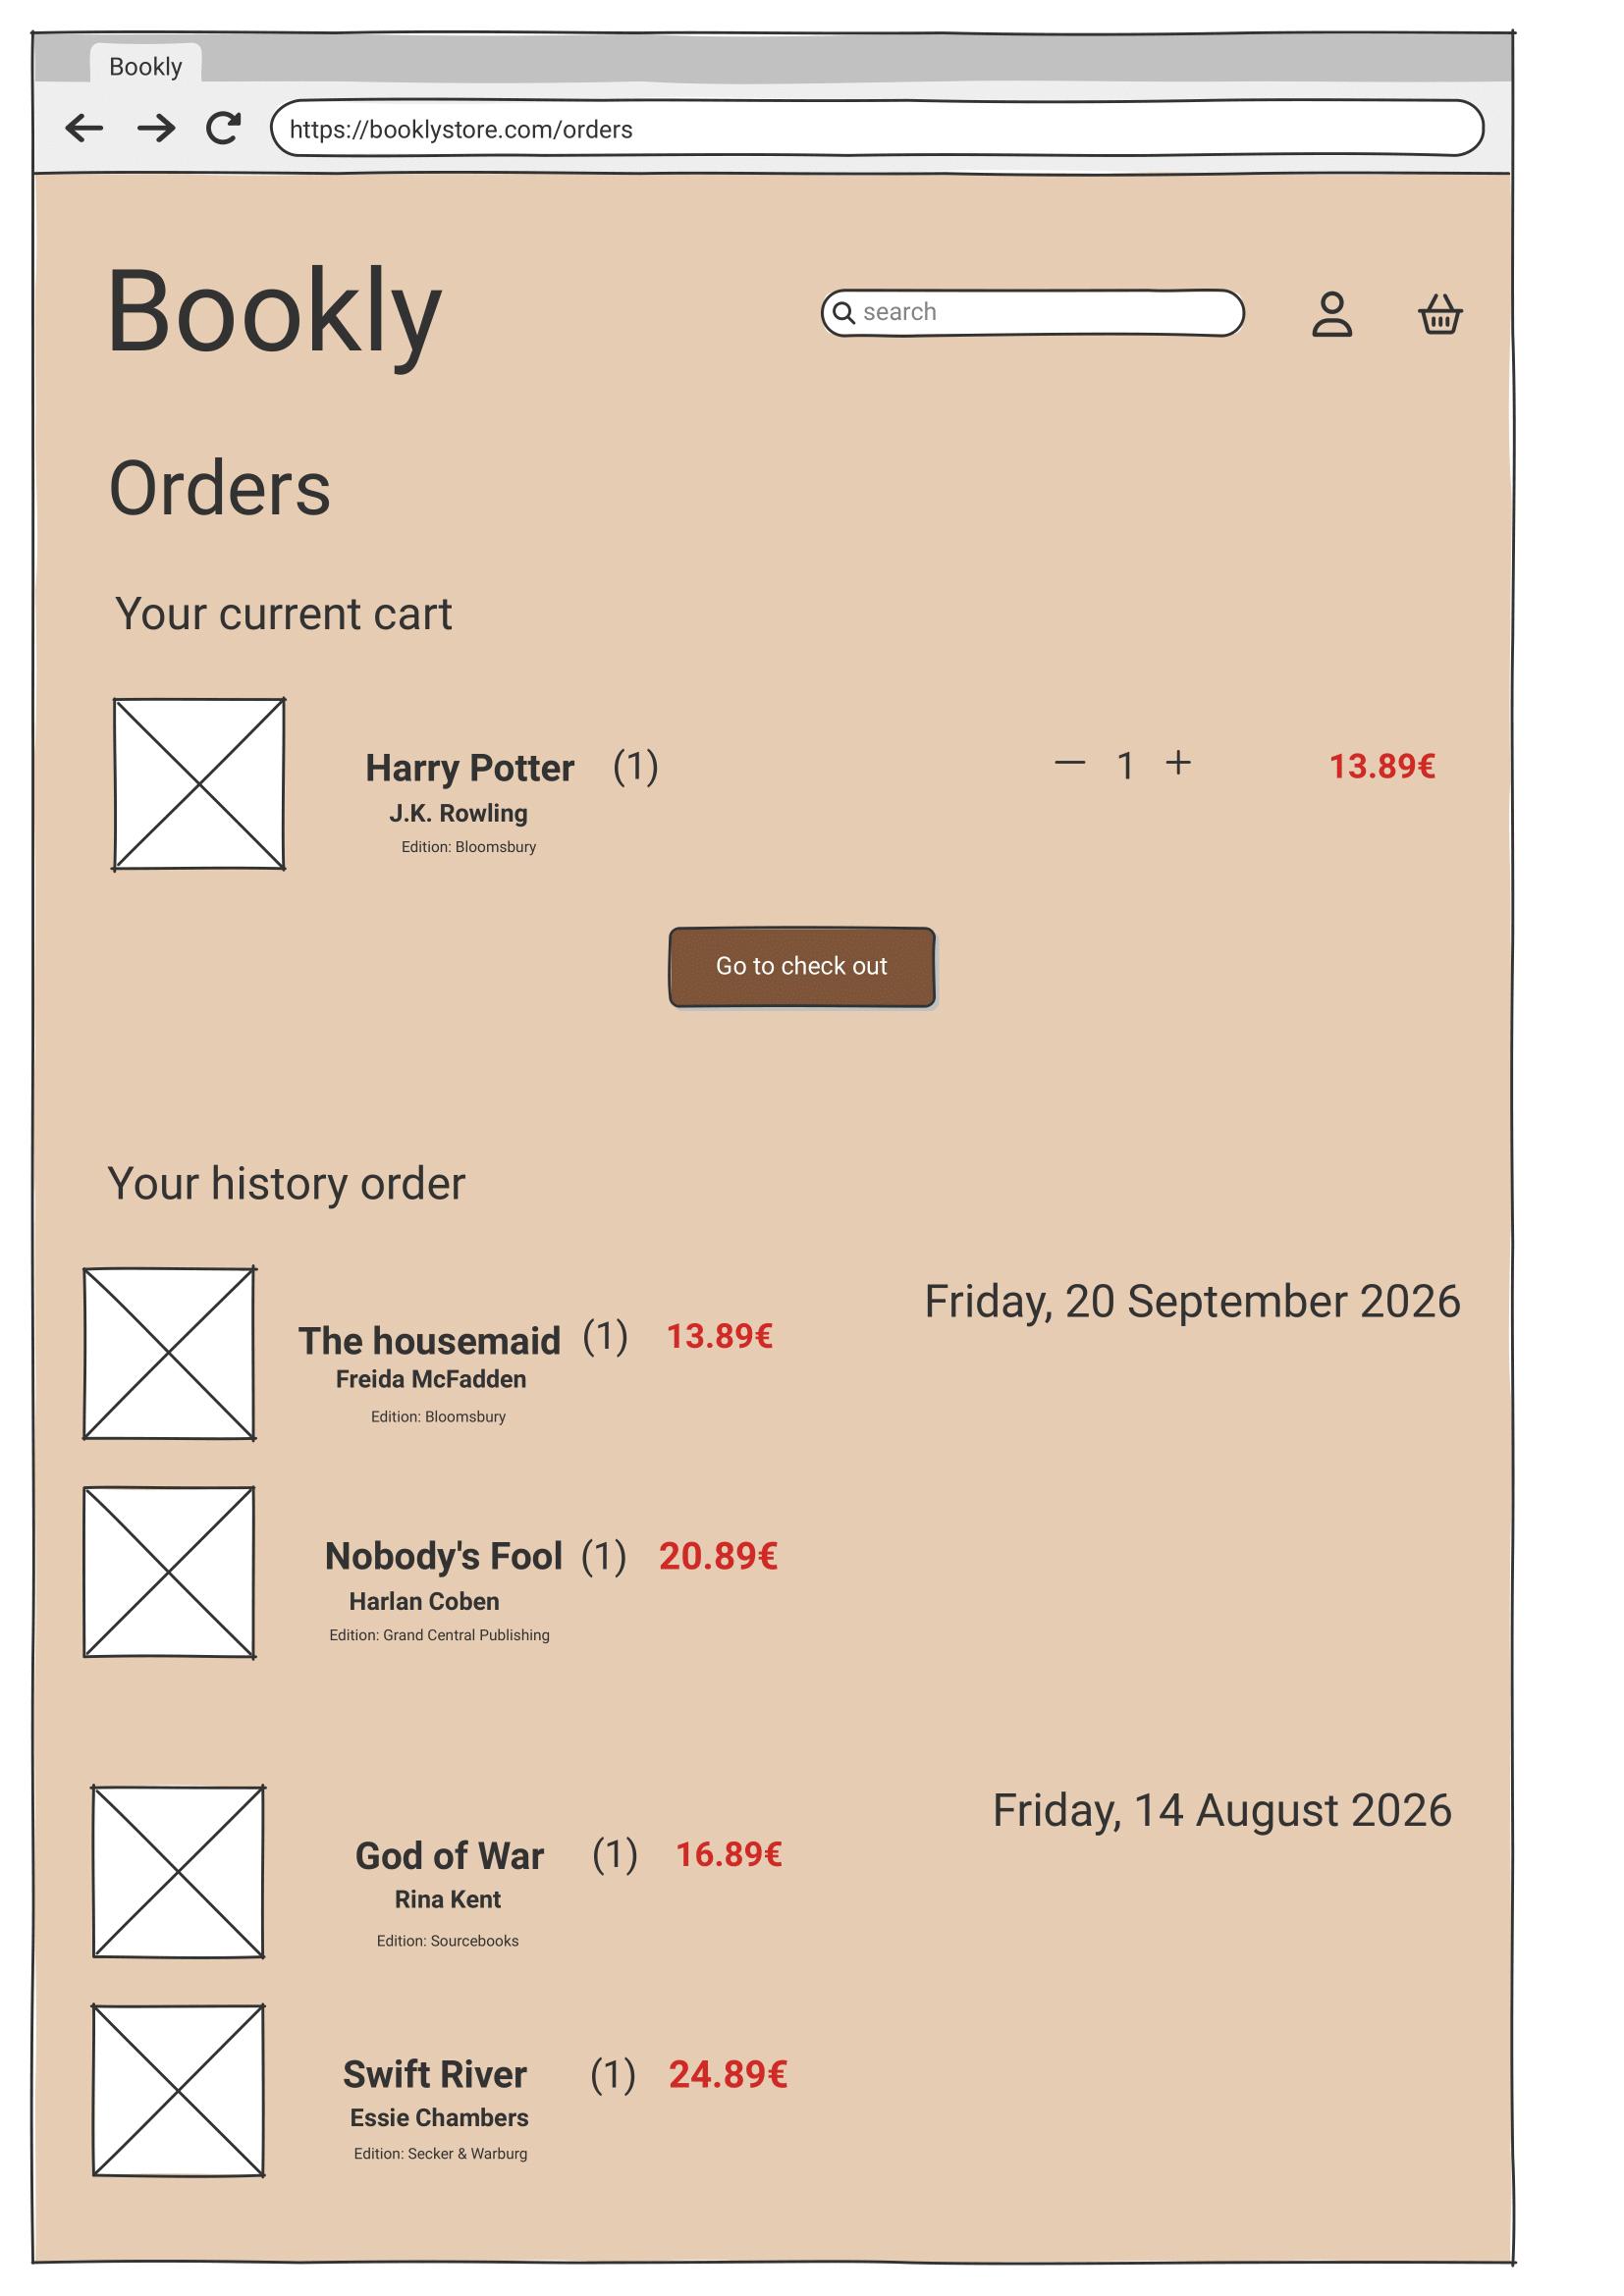
\includegraphics[width=0.6\linewidth]{HW1Report/photos/cartPage.png}

\begin{figure}[h!]
    \centering
    \caption{order page}
    \label{fig:enter-label}
\end{figure}
This page will present the contents of all the user's current shopping carts. It will include all books that the user has added, even if they haven't proceeded to checkout. The cart will persist between sessions for logged-in users. This page will also display the complete user's history order containing all the books the user has already ordered and the dates corresponding. 


\subsection{Wishlist Page} \label{sec:wishlist}
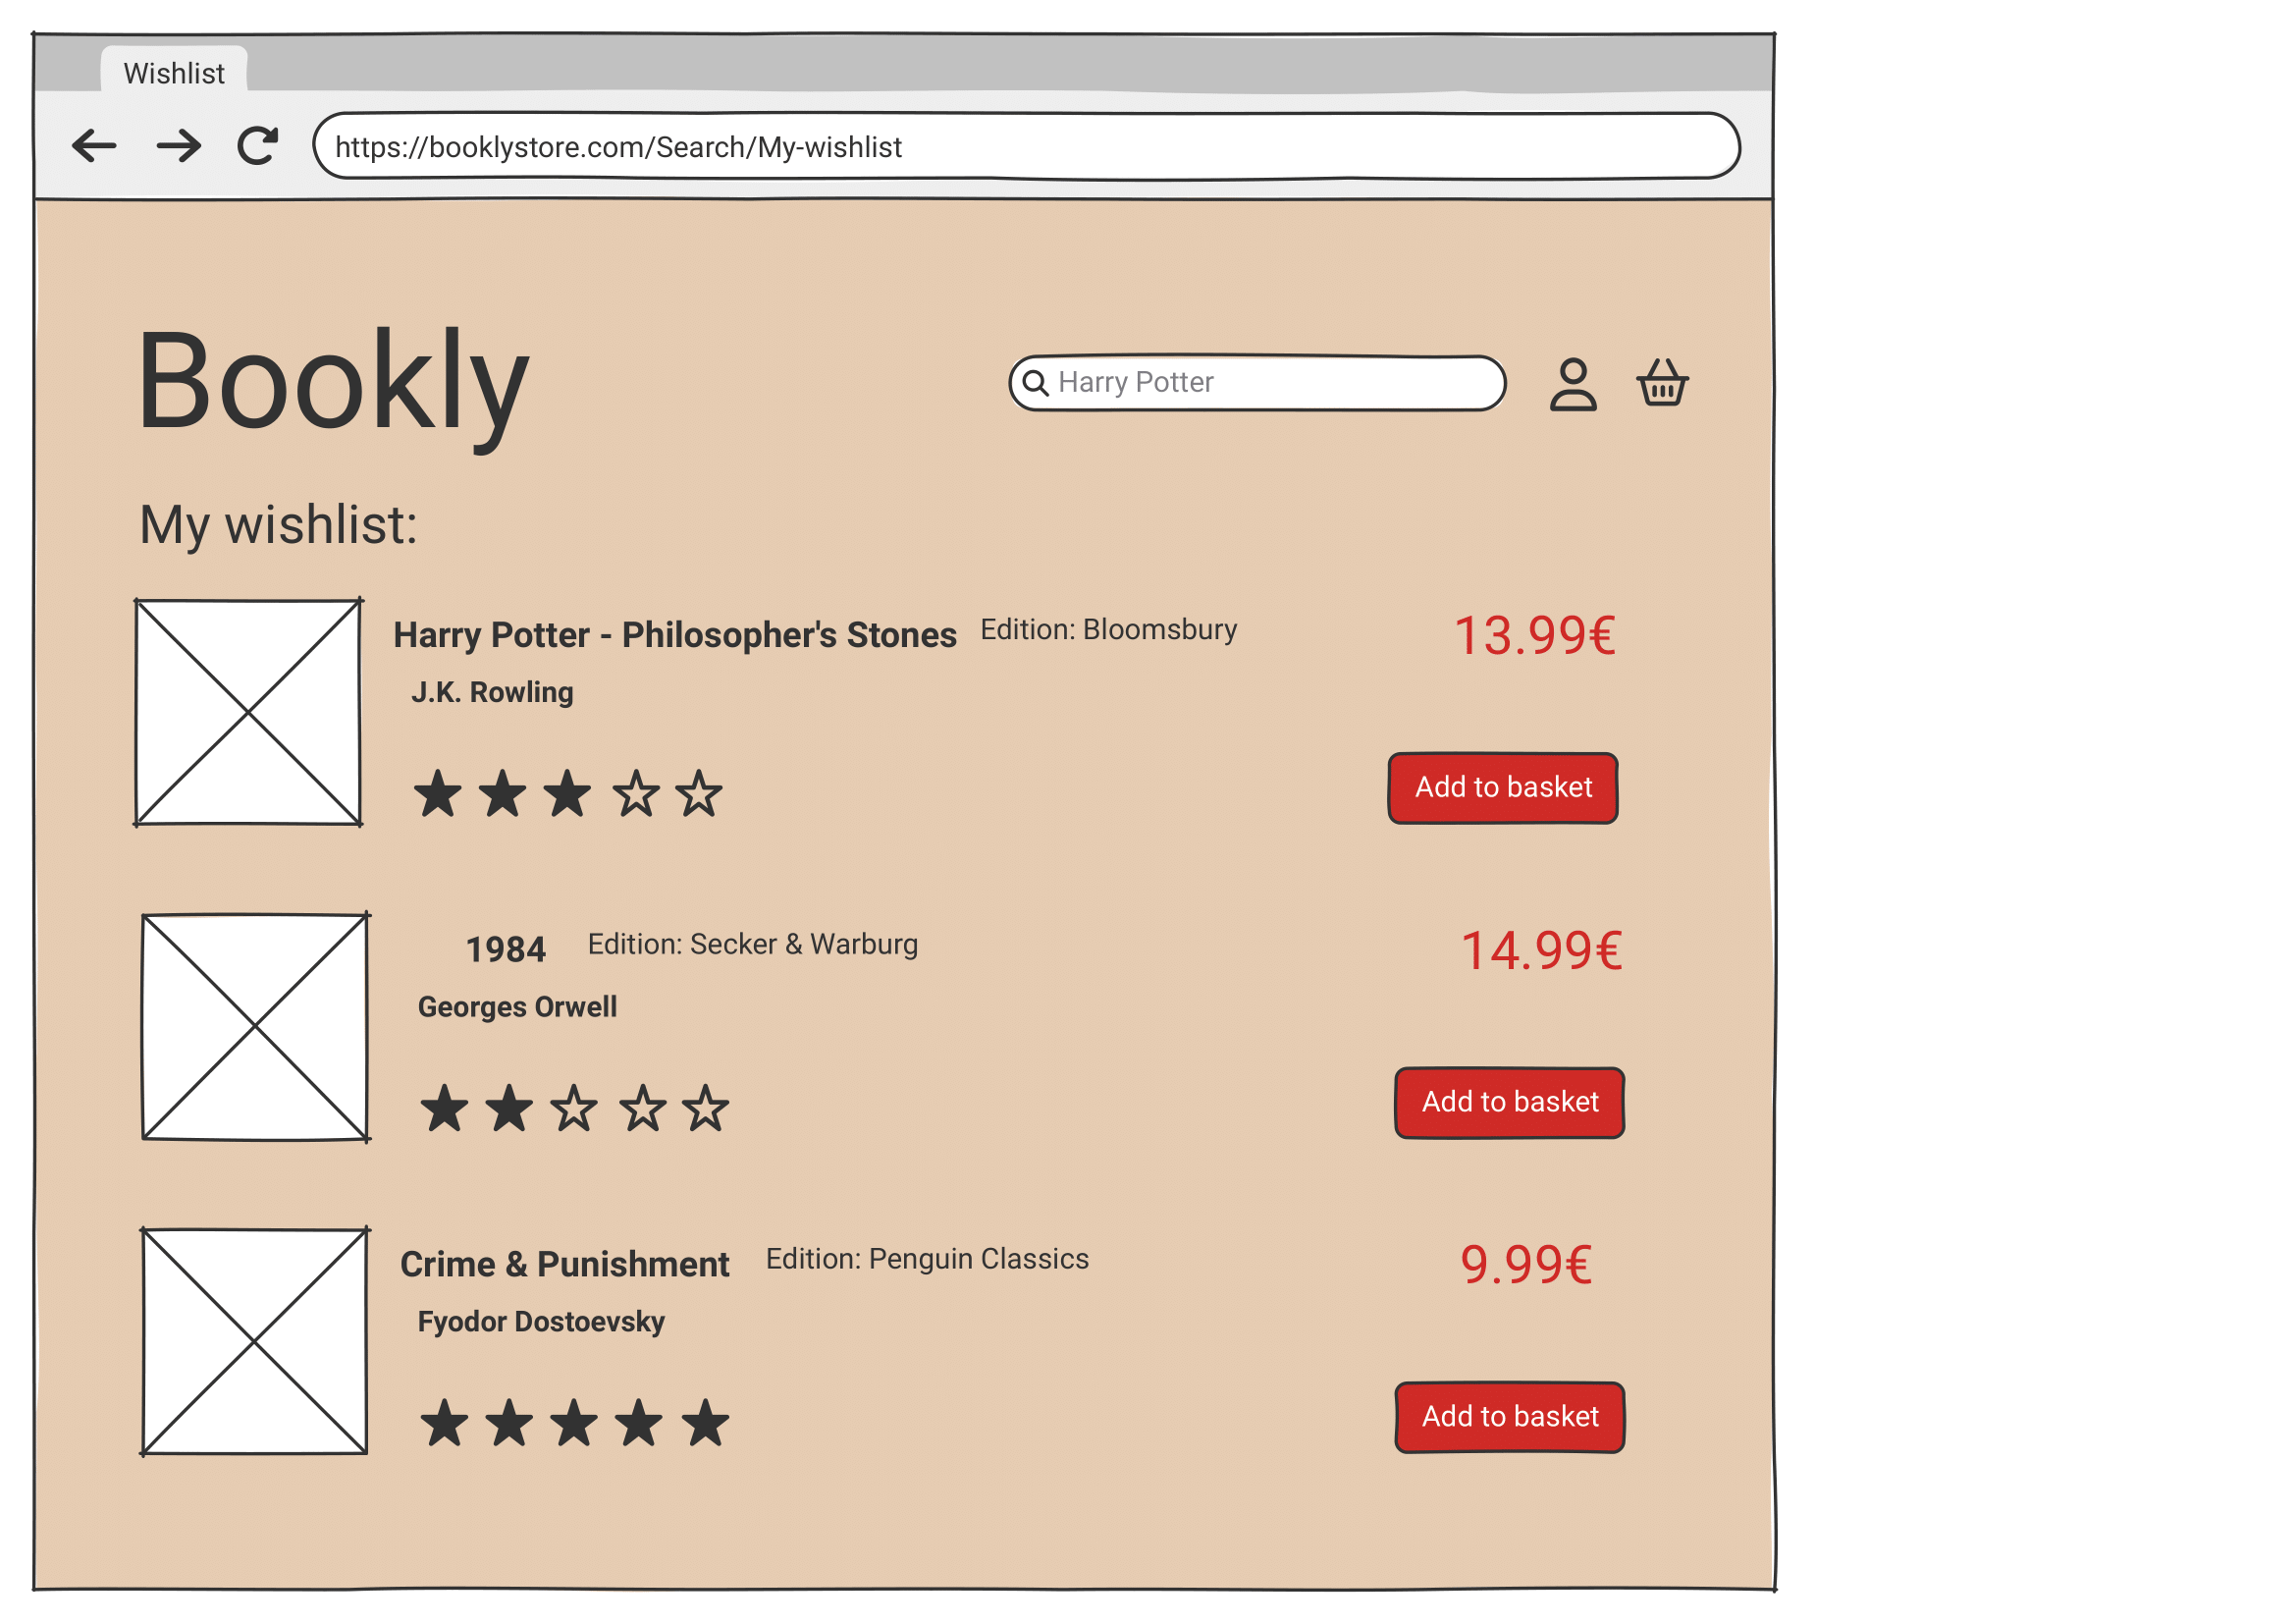
\includegraphics[width=0.6\linewidth]{HW1Report/photos/wishlist.png}

\begin{figure}[h!]
    \centering
    \caption{wishlist page}
    \label{fig:enter-label}
\end{figure}
The wishlist page displays all the books that the user has chosen to save for future reference. Users can move them directly into their basket from this page to initiate a purchase.